

\documentclass{article}
% Template-specific packages

\usepackage{graphicx} % Required for including images
\usepackage[hidelinks]{hyperref}
\usepackage{longtable}
\usepackage{epstopdf}
\usepackage{fullpage,enumitem,amsmath,amssymb,graphicx}
\usepackage{tikz}
\usepackage{pdfpages}
\usepackage{amsmath, amsthm}
\usepackage{fancyhdr}
\usepackage{siunitx}
\usepackage{mathtools}
\usepackage{mathrsfs}
\pagestyle{fancy}
\fancyhead[R]{\rightmark}
\fancyhead[L]{Ali BaniAsad 401209244}
\setlength{\headheight}{10pt}
\setlength{\headsep}{0.2in}
\usepackage{titling}
\usepackage{float}
\newcommand\Tstrut{\rule{0pt}{2.6ex}}         % = `top' strut
\newcommand\Bstrut{\rule[-0.9ex]{0pt}{0pt}}   % = `bottom' strut
%----------------------------------------------------------------------------------------
%	ASSIGNMENT INFORMATION
%----------------------------------------------------------------------------------------



%----------------------------------------------------------------------------------------
\usepackage{graphicx}
\title{Advanced Orbital Mechanics Project \\ Low-Thrust Transfer in a Multi-Body Environment using Reinforcement Learning}
\author{Ali BaniAsad 401209244}

\begin{document}
	\maketitle

\section{Introduction}
The objective of this project is to investigate the application of reinforcement learning (RL) techniques for low-thrust transfers in a multi-body environment. Orbital mechanics plays a crucial role in space exploration and satellite missions. Traditional methods for trajectory optimization often rely on assumptions of impulsive maneuvers, which may not be practical for missions with low-thrust propulsion systems. By leveraging RL algorithms, we aim to develop novel strategies for optimizing trajectories in complex gravitational fields.

\section{Problem Statement}
The problem can be defined as follows: given a spacecraft with a low-thrust propulsion system and a desired final orbital configuration, determine an optimal trajectory that minimizes the transfer time while satisfying various constraints such as fuel consumption, collision avoidance, and mission-specific objectives. This problem becomes more challenging in a multi-body environment, where gravitational interactions between celestial bodies significantly affect the spacecraft's trajectory.

\section{Approach}
To address this problem, we propose to use RL algorithms to learn optimal policies for spacecraft trajectory optimization. The RL agent will interact with a simulated environment that models the gravitational forces of the celestial bodies and the dynamics of the spacecraft. The agent will learn from the environment by iteratively selecting actions (thrust directions and magnitudes) to maximize cumulative rewards, which are designed to capture the desired objectives and constraints of the mission.

We will employ a model-free RL approach, specifically utilizing deep Q-networks (DQN), which have demonstrated success in complex control problems. The RL agent will receive inputs such as the spacecraft's state (position, velocity) and the current time, and output the optimal thrust direction and magnitude. The RL agent will be trained using a combination of techniques, including experience replay, target networks, and exploration-exploitation strategies, to ensure stable and efficient learning.

\section{Lyapunov Orbits}

Lyapunov orbits, named after the Russian mathematician Aleksandr Lyapunov, are a type of stable periodic orbit in celestial mechanics. These orbits exist in the restricted three-body problem, where the motion of a spacecraft is influenced by the gravitational forces of two larger celestial bodies, such as a planet and its moon.

In the circular restricted three-body problem (CRTBP), the primary body (e.g., the planet) and the secondary body (e.g., the moon) are assumed to follow circular orbits around their common center of mass. The spacecraft, considered as a massless particle, moves in the gravitational field generated by these two bodies. Lyapunov orbits are special trajectories that maintain a fixed orientation with respect to the primary and secondary bodies.

The position of a spacecraft in a CRTBP can be described using the Jacobi integral, denoted as $C$, which is a conserved quantity along the spacecraft's trajectory. The Jacobi integral is defined as:

\begin{equation}
C = \frac{1}{2} \left(\frac{{\dot{x}}^2 + {\dot{y}}^2 + {\dot{z}}^2}{G(m_1 + m_2)} - \Omega^2(x^2 + y^2) \right)
\end{equation}

where $(x, y, z)$ are the spacecraft's position coordinates, $(\dot{x}, \dot{y}, \dot{z})$ are the corresponding velocity components, $m_1$ and $m_2$ are the masses of the primary and secondary bodies, $G$ is the gravitational constant, and $\Omega$ is the angular velocity of the circular motion.

Lyapunov orbits correspond to critical points of the Jacobi integral, where the value of $C$ is constant. These orbits exist at certain energy levels and provide stable regions for spacecraft to orbit around the Lagrange points, which are stationary points in the CRTBP where the gravitational forces from the primary and secondary bodies balance each other.

The stability of Lyapunov orbits can be analyzed using linear stability analysis or numerical techniques. These orbits have been of great interest for space missions and satellite deployments, as they offer energy-efficient trajectories with long-term stability.

\section{Reference Trajectory (Heteroclinic Connection)}

In the field of dynamical systems and control theory, a reference trajectory refers to a desired path or trajectory that a system aims to follow. One interesting and important type of reference trajectory is the heteroclinic connection, which describes a connection between two or more equilibrium points of a dynamical system.

A heteroclinic connection is a trajectory that starts from one equilibrium point, passes through intermediate points or manifolds, and eventually reaches another equilibrium point. It represents a transition between different stable states of the system. The term "heteroclinic" refers to the fact that the trajectory crosses different stable manifolds corresponding to different equilibrium points.

Mathematically, a heteroclinic connection can be described by a set of differential equations that govern the dynamics of the system. The trajectory is typically obtained by solving these equations or by employing numerical methods. The connection between equilibrium points provides valuable insights into the behavior and stability of the system.

Heteroclinic connections have various applications in control theory, robotics, and physics. They can be utilized to design control strategies for transitioning between different operating modes or to achieve specific tasks. Additionally, they have been studied in the context of chaos and nonlinear dynamics, as they often exhibit intricate and interesting behaviors.

Understanding and analyzing heteroclinic connections require advanced mathematical tools and techniques, such as phase space analysis, stability analysis, and bifurcation theory. These tools help to elucidate the dynamics and properties of the reference trajectory.

In summary, a reference trajectory in the form of a heteroclinic connection represents a path that connects different equilibrium points of a dynamical system. It plays a crucial role in understanding the system's behavior, stability, and control. The study of heteroclinic connections contributes to the broader field of nonlinear dynamics and offers valuable insights into complex systems.

\section{Reinforcement Learning using MATLAB}

Reinforcement Learning (RL) is a subfield of machine learning that focuses on learning optimal decision-making policies through interaction with an environment. MATLAB provides a comprehensive framework for implementing and experimenting with RL algorithms.

\subsection{RL Toolbox in MATLAB}

MATLAB offers the RL Toolbox, a powerful set of functions and tools specifically designed for reinforcement learning tasks. The RL Toolbox provides a wide range of algorithms, such as Q-learning, SARSA, DQN (Deep Q-Network), and more. These algorithms can be applied to various RL problem domains, including control systems, robotics, finance, and games.

\subsection{Workflow for RL in MATLAB}

The typical workflow for implementing RL in MATLAB involves the following steps:

\begin{enumerate}
    \item Define the environment: Specify the environment in which the RL agent operates. This includes defining the state space, action space, and reward structure.
    
    \item Create the RL agent: Construct an RL agent using the appropriate algorithm from the RL Toolbox. Customize the agent's properties, such as exploration strategy and learning rate.
    
    \item Train the agent: Train the RL agent by interacting with the environment. The agent learns from the feedback it receives in the form of rewards and updates its policy accordingly. The RL Toolbox provides functions for carrying out the training process efficiently.
    
    \item Evaluate and fine-tune: Evaluate the trained agent's performance and fine-tune its parameters if needed. MATLAB provides tools for visualizing and analyzing the agent's behavior, allowing for iterative refinement of the RL approach.
    
    \item Deploy the agent: Once the RL agent achieves satisfactory performance, it can be deployed to perform tasks in real-world scenarios. MATLAB supports the deployment of RL agents to embedded systems, simulators, and physical environments.
\end{enumerate}

\subsection{Integration with Simulink and Stateflow}

MATLAB's RL capabilities can be seamlessly integrated with Simulink and Stateflow, which are powerful modeling and simulation environments. This integration enables the development of RL-based control systems and decision-making algorithms in complex dynamic systems.

By combining RL with Simulink and Stateflow, engineers and researchers can design and optimize controllers, autonomous systems, and robotic applications. The tight integration allows for a unified modeling and development environment, enabling efficient design iterations and system-level analysis.

MATLAB provides a comprehensive framework for implementing and experimenting with reinforcement learning algorithms. The RL Toolbox, along with its integration with Simulink and Stateflow, offers a powerful platform for developing RL-based control systems and decision-making algorithms. Researchers and engineers can leverage these capabilities to tackle a wide range of RL problems across various domains.

\section{Results}
First the Heteroclinic connection is found using the MATLAB code. The results are shown in Figure \ref{fig:hetcon}.
\begin{figure}[H]
	\centering
	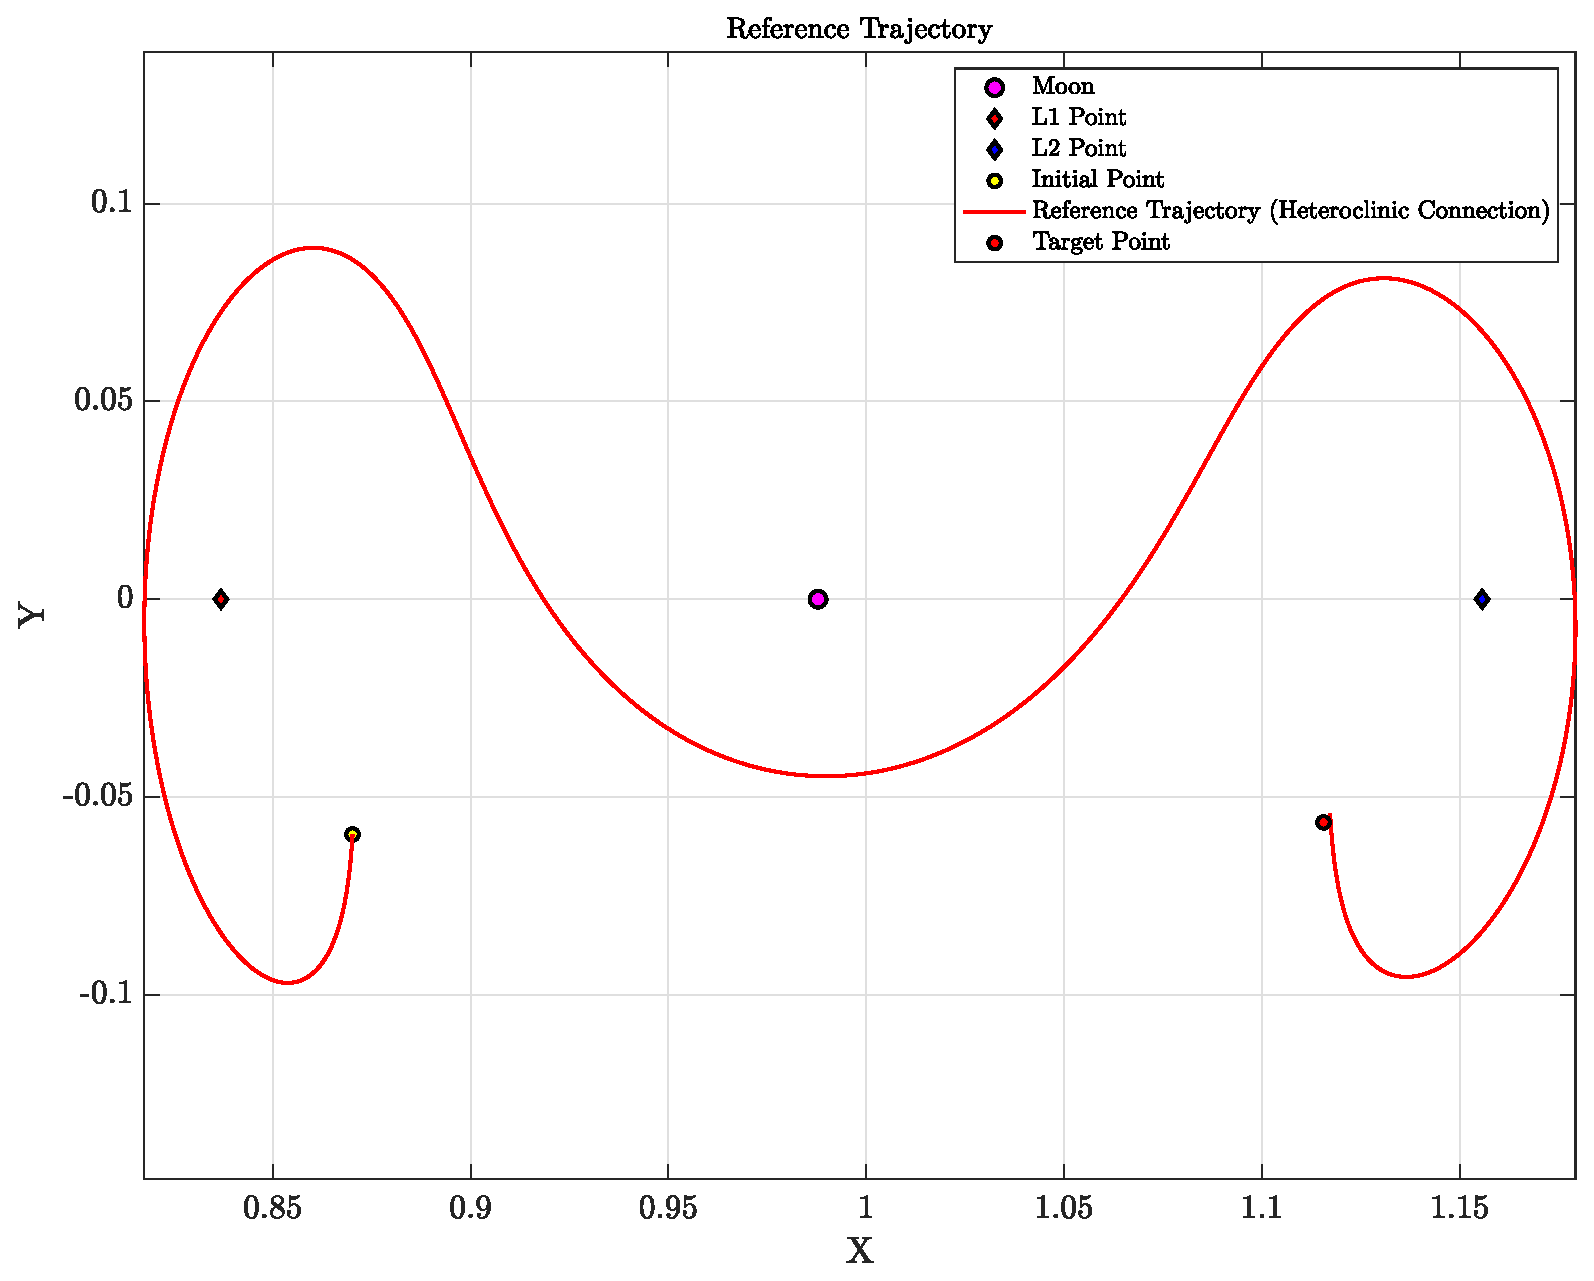
\includegraphics[width=\textwidth]{trajectory}
	\caption{Heteroclinic connection}
	\label{fig:hetcon}
\end{figure}
then used matlab to follow the trajectory using reinforcement learning. The results are shown below.
Two method is used one use only position observation and the other use both position and velocity observation.
here is training process for both methods.
\begin{figure}[H]
	\centering
	\includegraphics[width=\textwidth]{training.png}
	\caption{Training process}
	\label{fig:training}
\end{figure}
The results are shown in Figure \ref{fig:results}.
\begin{figure}[H]
	\centering
	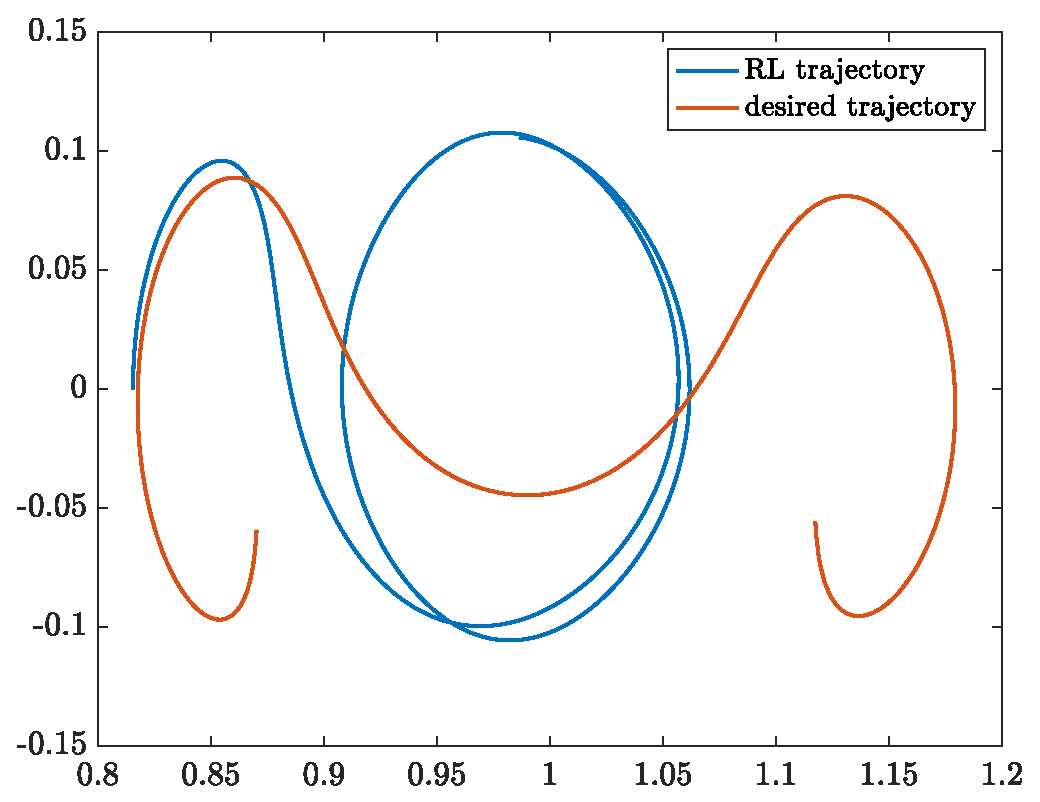
\includegraphics[width=\textwidth]{trajectory_RL}
	\caption{Results used RL}
	\label{fig:results}
\end{figure}



\section{Conclusion}
This project aims to explore the application of RL techniques for low-thrust trajectory optimization in a multi-body environment. By leveraging the power of RL algorithms, we seek to develop efficient and intelligent spacecraft trajectories that improve mission performance. The project's outcomes will contribute to the field of orbital mechanics and pave the way for future advancements in space exploration and satellite missions.


\end{document}

